\chapter{Agent--Based Data Augmentation for Fitting Stochastic Epidemic Models to Prevalence Data}
\label{chap:bda_for_fitting_sems_to_prevalence_data}

\section{Overview}
\label{sec:bda_overview}

Stochastic epidemic models (SEMs) are classic tools for modeling the spread of infectious diseases. A SEM represents the time evolution of an epidemic in terms of the disease histories of individuals as they transition through disease states. Incorporating stochasticity into epidemic models is important when the disease prevalence is low or when the population size is small. In both cases, the stochastic variability in the evolution of an epidemic greatly influences the probability of an outbreak, its severity, and the conclusions we draw about its dynamics \cite{keeling2008,allen2008introduction}. Moreover, many questions --- e.g., what is the final size distribution? What is the probability that a disease has been eradicated? --- cannot be answered using deterministic methods \cite{britton2010}.

The task of fitting a SEM is typically complicated by the limited extent of epidemiological data, which are recorded at discrete observation times, commonly describe just one aspect of the disease process, e.g., infections, and usually capture only a fraction of cases. Complete subject--level data, which would consist of the exact times at which individuals transition through disease states, are often unavailable \cite{oneill2010}. Fitting SEMs in the absence of complete subject--level data presents a complicated latent variable problem since it is usually impossible to analytically integrate over the missing data \cite{oneill2002}. This makes the observed data likelihood for a SEM intractable.

Agent--based data augmentation (DA) methods for fitting SEMs, first presented by \cite{oneill1999} and \cite{gibson1998}, target the joint posterior distribution of the missing data and model parameters to obtain a tractable complete data likelihood. That the augmentation is agent--based refers to the fact that subject--level disease histories, rather than population--level epidemic paths, are introduced as latent variables in the model. An advantage of the agent--based approach is that household structure and subject--level covariates may be incorporated into the model \cite{auranen2000,hohle2002,cauchemez2004bayesian, neal2004statistical,oneill2009}. Development of DA methods for SEMs is of continuing interest, and recent works by \cite{pooley2015}, \cite{QinShe15}, and \cite{shestopaloff2016sampling} have presented methods that could possibly be applied to epidemic count data. However, their algorithms forgo the flexibility of agent--based DA and, in the case of the latter two papers, have not been applied to SEMs.

We present an agent--based DA Markov chain Monte Carlo (MCMC) framework for fitting SEMs to time series count data. We obtain a tractable complete data likelihood by augmenting the data with subject--level disease histories. Our MCMC targets the joint posterior distribution of the latent epidemic process and the model parameters as we alternate between updating subject--level paths and model parameters. We propose each new subject--path, conditionally on the data, using a time--inhomogeneous continuous--time Markov chain (CTMC) with rates determined by the disease histories of the other individuals. These data--driven path proposals result in highly efficient perturbations to the latent epidemic path, and enable us to analyze epidemic count data in the absence of any subject--level information. In contrast, traditional agent--based DA MCMC algorithms rely on data--agnostic trans--dimensional proposals and suffer from convergence issues as the fraction of missing information becomes large \cite{roberts2001, mckinley2014simulation, pooley2015}. The \textit{de facto} need for some subject--level data has precluded the use of classical DA machinery in many settings. Thus, our MCMC algorithm enables exact Bayesian inference for SEMs fit to datasets that would have been impossible to study with existing agent--based DA methods. Our algorithm is not specific to any particular SEM dynamics or measurement process, and may be applied, with minimal modifications, to a broad class of SEMs. We apply our algorithm to disease prevalence data. Extensions to incidence count data are discussed, but are not explored in this dissertation.

\section{The data augmentation algorithm for an SIR model}
\label{sec:bda_sir_model}

For concreteness and clarity of exposition, we present our Bayesian DA algorithm (BDA) in the context of fitting a stochastic Susceptible--Infected--Recovered (SIR) model to binomially distributed prevalence counts. We also use our algorithm to fit Susceptible--Exposed--Infected--Recovered (SEIR) and Susceptible--Infected--Recovered--Susceptible (SIRS) models in Sections \ref{sec:bda_sir_seir_sirs_sim}, \ref{sec:bda_seir_misspec_sim}, and \ref{sec:_bda_app_bbs}, and outline the minimal adaptations required for these models in Section~\ref{sec:bda_seir_sirs_details}. We outline in Section~\ref{sec:bda_seir_sirs_details} the minimal adaptations required for fitting the Susceptible--Exposed--Infected--Recovered (SEIR) and Susceptible--Infected--Recovered--Susceptible (SIRS) models, which we demonstrate in Sections \ref{sec:bda_sir_seir_sirs_sim}, \ref{sec:bda_seir_misspec_sim}, and \ref{sec:bda_app_bbs}.

The SIR model describes the time evolution of an epidemic in terms of the disease histories of individuals as they transition through three states --- susceptible (S), infected/infectious (I), and recovered (R). Under simple SIR dynamics, each individual becomes infectious immediately upon becoming infected, and acquires lifelong immunity upon recovery. For simplicity, we assume that the population is closed and mixes homogeneously, and that there is no external force of infection. Therefore, the epidemic ceases once the pool of infectious individuals is depleted.

\subsection{Measurement process and data}
\label{subsec:bda_meas_proc}
Our data, $\bY = \lbrace Y_{1}, \dots, Y_L \rbrace$, are disease prevalence counts recorded at times $t_1,\dots,t_L \in [t_1,t_L]$. It should not beggar belief that the data could be subject to measurement error, for example underreporting in settings where asymptomatic individuals escape detection. Let $ S_\tau $, $ I_\tau $, and $ R_\tau $ denote the total susceptible, infected, and recovered people at time $ \tau $. We model the observed prevalence as a binomial sample, with constant mean case detection probability $ \rho $. Thus,
\begin{equation}\label{eqn:bda_emit_dist}
Y_\ell | I_{t_\ell},\rho \sim \mathrm{Binomial}\left (I_{t_\ell}, \rho\right ).\end{equation}

\subsection{Latent epidemic process}
\label{subsec:bda_pop_proc}
The data are sampled from a latent epidemic process, $ \bX = \lbrace \bX_1,\dots,\bX_N\rbrace $, that evolves continuously in time  as individuals become infected and recover. The state space of this process is $ \mcS = \lbrace S,I,R\rbrace^N $, the Cartesian product of $ N $ state labels taking values in $ \lbrace S,I,R\rbrace $. The state space of a single subject, $ \bX_j $, is $\mcS_j = \lbrace S, I, R\rbrace $, and a realized subject--path is of the form 
\begin{equation} \bx_j(\tau) = \left \lbrace \begin{array}{ll}
S\ ,& \tau < \tau^{(j)}_{\mathrm{I}},\\
I\ ,& \tau^{(j)}_{\mathrm{I}} \leq \tau < \tau^{(j)}_{\mathrm{R}},\\
R\ ,& \tau^{(j)}_{\mathrm{R}} \leq \tau,
\end{array} \right . \end{equation} 
where $ \tau^{(j)}_{\mathrm{I}} $ and $ \tau^{(j)}_{\mathrm{R}} $ are the infection and recovery times for subject $ j $ (though subject $ j $ may also never become infected or recover, or may become infected or recover outside of the observation period $ [t_1,t_L] $). We write the configuration of $ \bX $ at time $ \tau $ as $ \bX(\tau) = \left (\bX_1(\tau),\dots,\bX_N(\tau)\right ) $, and adopt the convention that $ \bX(\tau) $ and derived quantities, e.g., $ I_\tau $, depend on the configuration just before $ \tau $. We  use $ \tau^+ $ for quantities evaluated just after a particular time. The waiting times between transition events are taken to be exponentially distributed, and we denote by $ \beta $ and $ \mu $ the per--contact infectivity and recovery rates. Thus, the latent epidemic process evolves according to a time--homogeneous CTMC, with transition rate from configuration $ \bX $ to $ \bX^\prime $ given by
\begin{equation}
\lambda_{\bX,\bX^\prime} = \left \lbrace \begin{array}{rl}
\beta I,\ &\text{if } \bX\ \text{and } \bX^\prime\ \text{differ only in subject }j \text{, with }\bX_j=S\text{, and }\bX_j^\prime=I,\\
\mu,\ &\text{if } \bX\ \text{and } \bX^\prime\ \text{differ only in subject }j \text{, with }\bX_j=I\text{, and }\bX_j^\prime=R,\\
0,\ & \text{for all other configurations }\bX\ \text{and }\bX^\prime.
\end{array}\right.
\end{equation}
At the first observation time, we let $ \bX(t_1)|\bp_{t_1} \sim \mathrm{Categorical}\left (\lbrace S,I,R\rbrace, \bp_{t_1}\right ) $, where $ \bp_{t_1}=\left(p_{S}, p_{I},p_{R}\right) $ are the probabilities that an individual is susceptible, infected, or recovered. Let $ \btau = \lbrace\tau_0,\dots,\tau_{K+1}\rbrace $, where $ t_1 \equiv \tau_0 $ and $ t_L \equiv \tau_{K+1} $, be the (ordered) set of $ K $ infection and recovery times of all individuals along with the endpoints of the observation period $ [t_1,t_L] $. Let $ \ind{\tau_k \corresponds I} $ and $ \ind{\tau_k \corresponds R} $ indicate whether $ \tau_k $ is an infection or recovery time, and let $ \btheta = (\beta, \mu, \rho, \bp_{t_1}) $ denote the vector of unknown parameters. The complete data likelihood is 
\begin{align} 
\label{eqn:bda_comp_data_likelihood}
L(\bX, \bY | \btheta) &= \Pr(\bY|\bX, \rho)\times \Pr(\bX(t_1)|\bp_{t_1}) \times \pi(\bX |\bX(t_1),\beta, \mu) \nonumber \\
&=  \left [ \prod_{l = 1}^{L}\binom{I_{t_\ell}}{Y_\ell}  \rho^{Y_\ell}(1-\rho)^{I_{t_\ell} - Y_\ell}\right ] \times \left [p_{S}^{S_{t_1}} p_{I}^{I_{t_1}}p_{R}^{R_{t_1}}\right ]  \nonumber\\
&\hspace{0.2in} \times \prod_{k = 1}^{K}\left \lbrace \left [\beta I_{\tau_k}\times\ind{\tau_k \corresponds I} + \mu\times\ind{\tau_k \corresponds R}\right ] \exp{\left [-\left (\tau_k - \tau_{k-1}\right )\left (\beta I_{\tau_k} S_{\tau_k} + \mu I_{\tau_k}\right )\right ]}\right \rbrace \nonumber \\
& \hspace{0.2in} \times \exp \left [-\left (t_L - \tau_K\right )\left (\beta I_{\tau_K^+}S_{\tau_K^+} + \mu I_{\tau_K^+}\right )\right ]. 
\end{align}
We briefly reconcile what might seem like a discrepancy between the SIR model presented above and the lumped construction of the SIR model (see \cite{andersson2000stochastic}), which is common for a number of computational and analytical reasons. Our model describes the time evolution of the subject--level collection of disease histories, and thus evolves on the state space of individual disease labels. The lumped SIR model describes the time evolution of the vector of compartment counts, the state space of which is defined as the partition of the original state space obtained by aggregating the individuals in each of the model compartments. The lumped construction would have been appropriate had we chosen to augment the data with the compartment counts (for example, as in \cite{pooley2015}). Nonetheless, inference based on the full subject--level model will exactly match inference based on the lumped model. We discuss this further in Section \ref{sec:lumpability}.

\begin{figure}
	\centering
	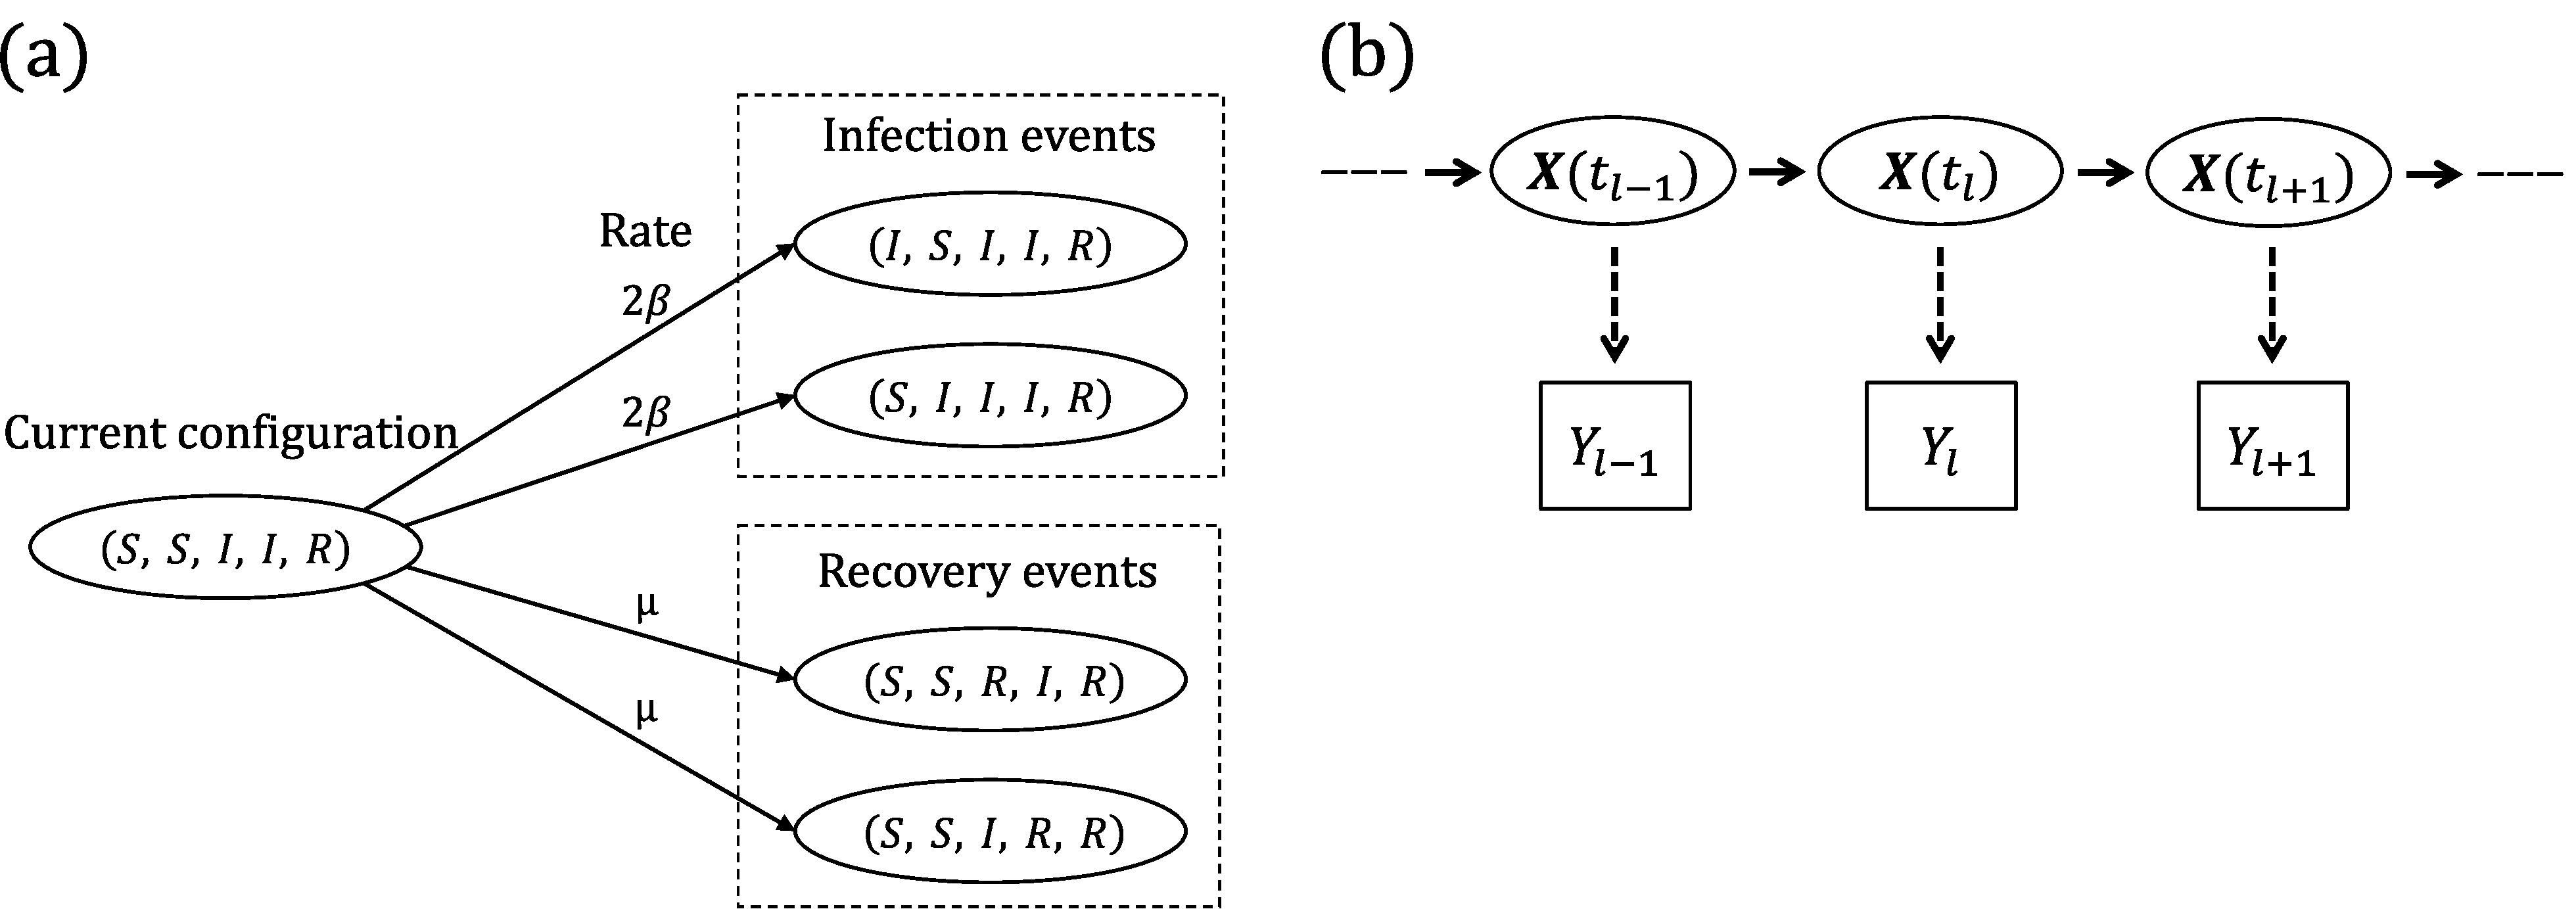
\includegraphics[width=0.95\linewidth]{figures/SIRdynamics_HMM}
	\caption{(a) SIR dynamics in a population of five subjects. The number of infecteds can increase from two to three via an infection of the first or second subject, reaching each of those configurations at rate $ 2\beta $. The number of recovered individuals can increase from one to two via a recovery of the third or fourth subject, reaching each of those configurations at rate $ \mu $. (b) Hidden Markov model for the joint distribution of the latent epidemic process and the data. The observations, $\mathbf{Y}_\ell,\ \ell=1,\dots,L$, are conditionally independent given $\bX(t)$, and $ \bY_\ell | I_{t_\ell}, \rho\sim\mathrm{Binomial}(I_{t_\ell}, \rho) $.}
	\label{fig:bda_SIRdynamics_HMM}
\end{figure}

\subsection{Subject--path proposal framework}
\label{subsec:bda_subj_proc}
The observed data likelihood in the posterior  $ \pi(\btheta|\bY) \propto \pi(\bY|\btheta)\pi(\btheta)=\int L(\bY|\bX, \btheta) \pi(\bX|\btheta) \pi(\btheta) \mathrm{d}\pi(\bX)$
is analytically intractable for even moderately sized $ N $ as it involves a  high dimensional integral over the collection of subject--paths, $ \bX $. The strategy employed in DA methods is to introduce the subject--paths, $ \bX $, as latent variables in the model. This enables us to work with the tractable complete data likelihood given by (\ref{eqn:bda_comp_data_likelihood}). The joint posterior distribution is \begin{equation}
\label{eqn:bda_jointpost}
\pi(\btheta, \bX| \bY) \propto \Pr(\bY|\bX,\rho) \times\pi(\bX|\bX(t_1),\beta,\mu) \times \Pr\left (\bX(t_1)|\bp_{t_1}\right) \times\pi(\beta)\pi(\mu) \pi(\rho) \pi(\bp_{t_1}),
\end{equation} where $ \pi(\beta)$, $\pi(\mu)$, $\pi(\rho)$, and $\pi(\bp_{t_1}) $ are prior densities. Our MCMC targets the joint posterior distribution, given by (\ref{eqn:bda_jointpost}), as we alternate between updating $ \bX|\btheta,\bY $ and $ \btheta|\bX,\bY $. 

Given the current collection of subject--paths, $ \xcur $, we propose $ \xnew $ by sampling the path of a single subject $\bX_j$, conditionally on the data, using a time--inhomogeneous CTMC with state space $ \mcS_j  $ and rates conditioned on the collection of disease histories of other individuals, $ \bx_{(-j)}  = \lbrace \bx_1,\dots,\bx_{j-1},\bx_{j+1},\dots,\bx_N \rbrace$. The proposed collection of paths is accepted or rejected in a Metropolis--Hastings step. 

Let $ \btau^{(j)} = \lbrace \tau_\mathrm{I}^{(j)},\tau_\mathrm{R}^{(j)}\rbrace $ be the (possibly empty) set of infection and recovery times for subject $ j $, and define $ \btau^{(-j)} = \lbrace\btau\setminus\btau^{(j)}\rbrace = \left \lbrace \tau_0^{(-j)} ,\tau_1^{(-j)}, \dots, \tau_{M}^{(-j)}, \tau_{M+1}^{(-j)}\right \rbrace$, where $ t_1 \equiv \tau_0^{(-j)} $ and $ t_L\equiv\tau_{M+1}^{(-j)} $, to be the set of $ M\leq K $ (ordered) times at which other subjects become infected or recover, along with $ t_1$ and $ t_L $. Let $ \mcI = \lbrace \mcI_1, \dots,\mcI_{M+1}\rbrace $ be the intervals that partition $ [t_1,t_L]$, i.e. $ \mcI_1 = \left [\tau_0^{(-j)},\tau_1^{(-j)}\right ),\ \mcI_2=\left [\tau_1^{(-j)},\tau_2^{(-j)}\right ),\dots,\ \mcI_{M+1}=\left [\tau_{M}^{(-j)},\tau_{M+1}^{(-j)}\right )$. Let $ I_\tau^{(-j)} = \sum_{i\neq j}\ind{\bX_i(\tau) = I} $ be the prevalence at time $ \tau $, excluding subject $ j $. Let $ \bLambda^{(-j)}(\btheta) = \left \lbrace\bLambda_1^{(-j)}(\btheta),\dots,\bLambda_{M+1}^{(-j)}(\btheta) \right \rbrace$ be the sequence of rate matrices corresponding to each interval in $ \mcI $, where for $ m=1,\dots,M+1 $,
\begin{equation} \bLambda_m^{(-j)}(\btheta) = \bordermatrix{ & S & I & R \cr
	S & -\beta I_{\tau_m}^{(-j)} & \beta I_{\tau_m}^{(-j)} & 0 \cr 
	I & 0 & -\mu & \mu \cr
	R & 0 & 0 & 0 }.
\end{equation}

We can construct the transition probability matrix for subject $ j $ over interval $ I_m $, $$ \bP^{(j)}(\tau_{m-1},\tau_m) = \left (
p_{a,b}^{(j)}(\tau_{m-1},\tau_m)\right )_{a,b\in \mcS_j}, $$ where $ p_{a,b}^{(j)}(\tau_{m-1},\tau_m) = \Pr(\bX_j(\tau_m)=b|\bX_j(\tau_{m-1})=a, \btheta) $, using the matrix exponential $$
	\bP^{(j)} (\tau_{m-1},\tau_m)= \exp\left [(\tau_m - \tau_{m-1})\bLambda^{(-j)}_m(\btheta)\right ].
	$$
This computation requires an eigen--decomposition of each rate matrix. We may reduce the total computational burden by computing the eigen decompositions analytically, and by caching the decompositions to avoid duplicate computations. One additional point is that while the eigen--values of any SIR rate matrix are always real valued, this is not generally true, e.g., it is possible for the rate matrix of an SIRS model to have complex eigenvalues. In this case, we obtain a real valued transition probability matrix by first applying a rotation to each rate matrix with complex eigenvalues to obtain its real canonical form \cite{hirsch2013differential}. This is discussed in Section \ref{sec:mtx_exp}.

By the Markov property, the time--inhomogeneous CTMC density over the observation period $ [t_1,t_L] $, denoted $ \pi(\bX_j | \bx_{(-j)}, \btheta) \equiv \pi\left (\bX_j | \bLambda^{(-j)}(\btheta); \mathcal{I}\right ) $, can be written as a product of time--homogeneous CTMC densities over the inter--event intervals $ \mcI_1,\dots,\mcI_{M} $. Thus,
\begin{equation}
\label{eqn:subj_level_dens}
\pi\left (\bX_j | \bLambda^{(-j)};\mathcal{I}\right ) = \Pr(\bX_j(t_1) | \bp_{t_1}) \prod_{m=1}^{M}\pi\left (\bX_j  | \bx_j(\tau_{m-1}), \bLambda^{(-j)}_m(\btheta);\mcI_m\right ).
\end{equation} 
Similarly, the transition probability matrix over an interval $ \mathcal{I}_\ell = [t_{\ell-1},t_\ell] $ can be written as the product of transition probability matrices over the sub--intervals in $ \mathcal{I}_\ell $, within which the subject--level CTMC is time--homogeneous. Thus, the transition probability matrix over an inter--observation interval, $ \mcI_\ell = [t_{\ell-1}, t_\ell] $, partitioned by $ S $ transition events that define inter--event intervals with endpoints given by times $ t_{\ell-1} \equiv \tau_{\ell,0}^{(-j)} < \tau_{\ell,1}^{(-j)}<\dots<\tau_{\ell,S-1}^{(-j)}  < \tau_{\ell,S}^{(-j)} \equiv t_\ell $, is constructed as
\begin{equation*}\label{eqn:inhomog_tpmprod} \bP^{(j)}(t_{\ell - 1},t_\ell) = \prod_{s=1}^{S}\bP^{(j)}\left(\tau_{\ell,s-1}^{(-j)},\tau_{\ell,s}^{(-j)}\right) .\end{equation*}

The MCMC algorithm for constructing a subject--path proposal proceeds in three steps (Figure \ref{fig:sampling_diagram}):  
\begin{enumerate}[nolistsep]
	\item \textit{HMM step}: sample the disease state of the subject under consideration at the observation times, conditional on the data and disease histories of other subjects.
	\item \textit{Discrete time skeleton step}: sample the state at times when the time--inhomogeneous CTMC rates change, conditional on the states sampled in the HMM step. 
	\item \textit{Event time step}: sample the exact times of transition events conditional on the sequence of states sampled in the previous steps. 
\end{enumerate}

\begin{figure}[ht!]
	\centering
	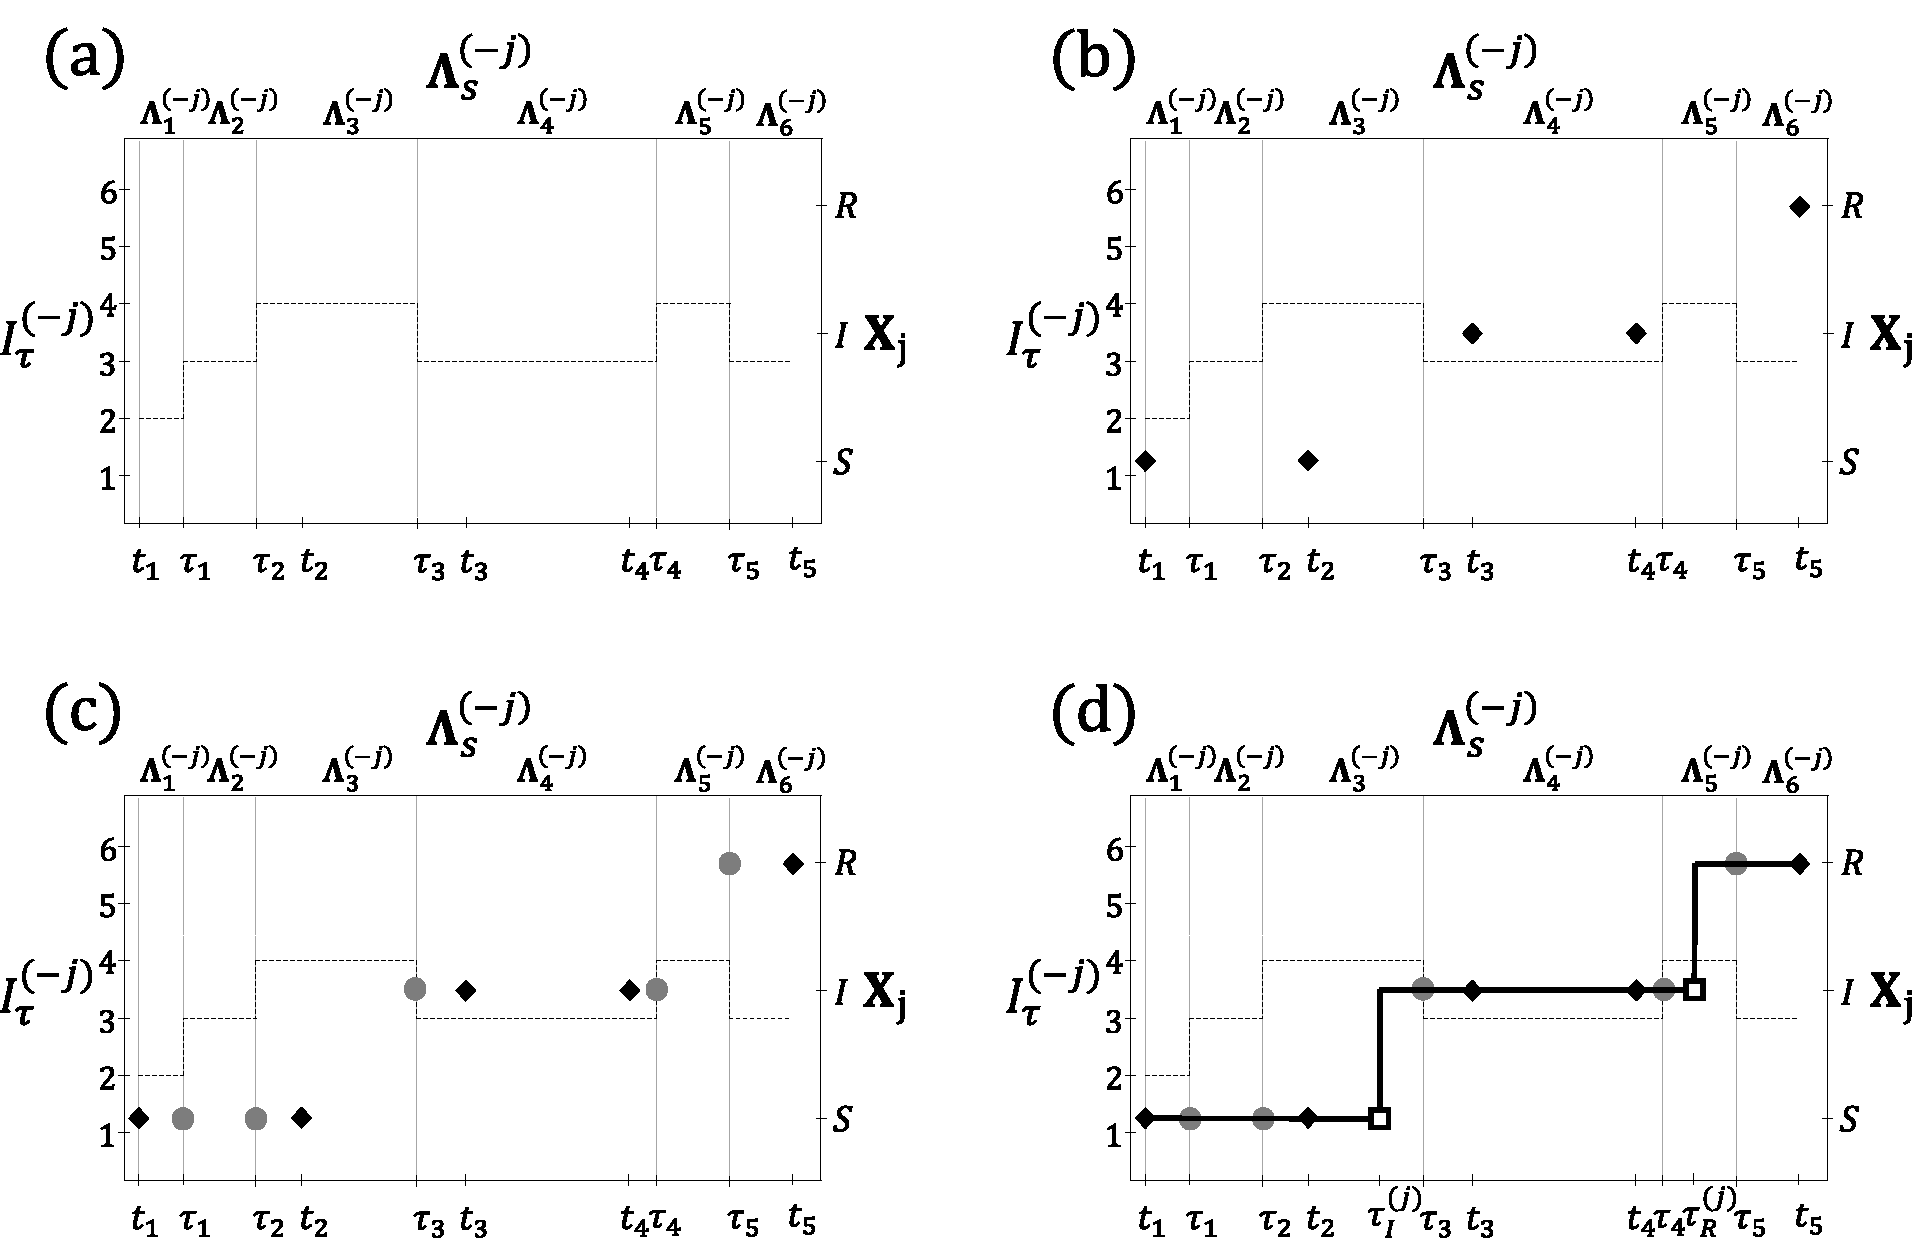
\includegraphics[width=0.95\linewidth]{figures/sampling_diagram.pdf}
	\caption{Procedure for constructing a subject--path proposal with SIR dynamics. (a) The dashed line depicts the number of infected individuals, excluding $ \bX_j $, the subject whose path is being sampled. The observation times, $ t_1,\dots,t_5 $, and times at which other subjects change disease states, $ \tau_1,\dots,\tau_5 $, are shown on the bottom axis. Rate matrices of the time--inhomogeneous CTMC (top axis) are constant within inter--event intervals (vertical lines). The state space of the subject--level process, $ \bX_j $, is shown on the right axis. (b) \textit{HMM step}: Sample the state of $ \bX_j $ at $ t_1,\dots,t_5 $, conditional on the data and on the disease histories of other subjects. (c) \textit{Discrete time skeleton step}: Sample the infection status at  $ \tau_1,\dots,\tau_5 $, conditional on the sequence of states sampled in the HMM step. (d) \textit{Event time step}: Sample the infection and recovery times from endpoint-conditioned time--homogeneous CTMC distributions, conditional on the sequence of disease states sampled in the HMM and discrete time skeleton steps.}
	\label{fig:sampling_diagram}
\end{figure}

\subsubsection{HMM step}
The key to sampling a sequence of disease states at the observation times is to rewrite the emission probability, given by (\ref{eqn:emit_dist}), as
\begin{equation}\label{eqn:hmm_emit}
Y_\ell| X_j(t_\ell), I_{t_\ell}^{(-j)},\rho \sim \mathrm{Binomial}\left (\ind{X_j(t_\ell)=I} + I_{t_\ell}^{(-j)}, \rho\right ).
\end{equation}
The emission probability in (\ref{eqn:hmm_emit}) only depends on whether subject $ j $ is infected at time $ t_\ell $, since we treat the paths of all other subjects, and the parameters, as fixed. Furthermore, the data are conditionally independent of one another, given $ \bx$ and $ \btheta $, which induces a hidden Markov model (HMM) over the joint distribution $ \bX $ and $ \bY $ (Figure \ref{fig:SIRdynamics_HMM.eps}b). 

We sample the discrete path of $ \bX_j $ at times $ t_1,\dots,t_L $ from the conditional distribution of $ \bX_j $, denoted $ \pi(\bX_j | \bY,\bx_{(-j)}, \btheta; t_1,\dots,t_L) $, using the stochastic forward--backward algorithm \cite{scott2002}. The algorithm enables us to efficiently sample from $ \pi\left (\bX \mid \bY, \bX_{(-j)}, \btheta\right ) $ by recursively accumulating, in a ``forward'' pass, information about the probability of various paths through $ \mcS $, conditional on the data, and then recursively sampling a trajectory in a ``backwards'' pass. 

In the forward recursion, we construct a sequence of matrices $ \bQ^{(t_2)}_j,\dots,\bQ^{(t_L)}_j $, where $ \bQ^{(t_\ell)}_j = \left (q_{j,r,s}^{(t_\ell)}\right )$, and $ q_{j,r,s}^{(t_\ell)} = \Pr\left (\bX_j(t_\ell) = s, \bX_j(t_{\ell - 1}) = r \mid \bY_{t_1}^{t_{\ell}},\bX_{(-j)},\btheta \right )$. Let $ \bP^{(j)}_{r,s}(t_{\ell - 1},t_\ell) = \Pr\left (\bX_j(t_\ell) = s \mid \bX(t_{\ell-1})=r, \btheta; \bX_{(-j)}\right ) $. If there are changes in the numbers of infected individuals in interval $ \mathcal{I}_\ell $, we construct the transition probability matrix for that interval as in (\ref{eqn:inhomog_tpmprod}). Then, 
\begin{equation}
q_{j,r,s}^{(t_\ell)} \propto \pi_{j}^{(t_\ell)}\left (r \mid \bX_{(-j)}, \btheta\right ) \times \bP^{(j)}_{r,s}\left (t_{\ell-1},t_\ell\right ) \times f\left (Y_{t_\ell} \mid \bX_j(t_\ell),\bX_{(-j)}(t_\ell), \rho, \bp_{t_1}\right ),	
\end{equation}
where $  \pi_{j}^{(t_\ell)}\left (r \mid \bX_{(-j)}, \btheta, \rho\right ) = \sum_r q_{j,r,s}^{(t_j)}$ and with proportionality reconciled via $ \sum_r\sum_s q_{j,r,s}^{(t_j)}=1 $.

In the backwards recursion, we sample the sequence of states at times $ t_1,\dots,t_L $ from the distribution $ \pi\left (\bX \mid \bY, \bX_{(-j)},\btheta, \rho,\bp_{t_1}\right )$. To do this, we first note that\vspace{-0.25in}

\begin{scriptsize}
	\begin{align*}\scriptsize
	\pi\left (\bX \mid \bY, \bX_{(-j)},\btheta, \rho,\bp_{t_1}\right ) &= \pi\left (\bX_j(t_L) \mid \bY_{t_1}^{t_L}, \bX_{(-j)},\btheta,\rho, \bp_{t_1}\right ) \prod_{\ell = 1}^{L-1}\pi \left (\bX_j(t_{L-\ell}) \mid \bX_{j,t_{L-\ell+1}}^{t_L}, \bX_{(-j)}, \bY_{t_1}^{t_L}, \btheta, \rho, \bp_{t_1}\right )\\
	&= \pi\left (\bX_j(t_L) \mid \bY_{t_1}^{t_L}, \bX_{(-j)},\btheta,\rho, \bp_{t_1}\right ) \prod_{\ell = 1}^{L-1}\pi \left (\bX_j(t_{L-\ell}) \mid \bX_{j,t_{L-\ell+1}}, \bX_{(-j)}, \bY_{t_1}^{t_{L-\ell+1}}, \btheta, \rho, \bp_{t_1}\right ),
	\end{align*}
\end{scriptsize} 
where the second equality follows from the conditional independence of the HMM. We proceed by first drawing $ \bX_j(t_L) $ from $ \pi_j^{(t_L)}\left (\cdot \mid \bX_{(-j)}, \btheta,\rho\right  ) $, and then drawing $ \bX_j(t_\ell),\ \ell = L-1,\dots,1, $ each in turn from the categorical distribution with masses proportional to column $ \bx_j(t_{\ell+1}) $ of $ \bQ_j^{(t_{\ell+1})} $. 

\subsubsection{Discrete-time skeleton step}
It would be straightforward to sample the exact infection and recovery times of subject $ j $, conditional on the sequence of states at times $ t_1,\dots, t_L $, if the subject--level CTMC rates did not possibly vary over each inter--observation interval. We may reduce our problem to the time--homogeneous case by first sampling the disease state at the intermediate event times when the CTMC rates change, and then sampling the full path within each inter--event interval. Consider an inter--observation interval, $ \mcI_\ell = [t_{\ell-1}, t_\ell] $, containing inter--event intervals whose endpoints are given by times $ t_{\ell-1} \equiv \tau_{\ell,0}^{(-j)} < \tau_{\ell,1}^{(-j)}<\dots<\tau_{\ell,n-1}^{(-j)}  < \tau_{\ell,n}^{(-j)} \equiv t_\ell $. We recursively sample $ \bX_j $ at each intermediate event time, beginning at $ \ttau_1 $, from the discrete distribution with masses 
\begin{align}
&\Pr\left (\bX_j\left (\ttau_{i}\right ) = x_{i} \mid  \bX_j\left (\ttau_{i-1}\right ) = x_{i-1}, \bX_j\left (\ttau_{n}\right ) = x_n\right ) \nonumber \\  &\hspace{1in}= \frac{\Pr\left (\bX_j\left (\ttau_{i}\right ) = x_{i}, \bX_j\left (\ttau_{i-1}\right ) = x_{i-1}, \bX_j\left (\ttau_{n}\right ) = x_n\right )}{\Pr\left (\bX_j\left (\ttau_{i-1}\right ) = x_{i-1}, \bX_j\left (\ttau_{n}\right ) = x_n\right )} \nonumber\\
&\hspace{1in}= \frac{\Pr\left (\bX_j\left (\ttau_{i}\right ) = x_{i} \mid \bX_j\left (\ttau_{i-1}\right ) = x_{i-1}\right )\Pr\left (\bX_j\left (\ttau_{n}\right ) = x_n \mid \bX_j\left (\ttau_{i}\right ) = x_{i}\right )}{\Pr\left (\bX_j\left (\ttau_{n}\right ) = x_n | \bX_j\left (\ttau_{i-1}\right ) = x_{i-1}\right)} \nonumber\\
&\hspace{1in} = \frac{\left [\bP^{(j)}\left (\ttau_{i-1},\ttau_{i}\right )\right ]_{x_{i-1},x_{i}}\left [\prod_{k=i}^{n-1}\bP^{(j)}\left (\ttau_{k}, \ttau_{k+1}\right )\right ]_{x_{i},x_n}}{\left [\prod_{k=i-1}^{n-1}\bP^{(j)}\left (\ttau_{k}, \ttau_{k+1}\right )\right]_{x_{i-1},x_n}}.
\label{eqn:dt_skel}
\end{align}

\subsubsection{Event time step}
The final step in constructing a subject--path is to sample the exact infection and recovery times given the discrete sequence of states obtained in the previous two steps. This amounts to simulating the path of an endpoint--conditioned time--homogeneous CTMC, a task for which there exist a variety of efficient methods \cite{hobolth2009}. When fitting the SIR model, we chose to use modified rejection sampling, a modification of Gillespie's direct algorithm \cite{gillespie1976} that explicitly avoids simulating constant paths. This method is known to be efficient when the states differ at the endpoints of small time intervals. We used uniformization--based sampling \cite{hobolth2009} when fitting SEIR and SIRS models, which was more robust when sampling paths in intervals with multiple transitions. Fast implementations of these methods are available in the \texttt{ECctmc} package in \texttt{R} \cite{ECctmc}. We briefly summarize the algorithms below, but to \citet{hobolth2009} for a more thorough discussion.   

Our goal is to simulate a path for a time--homogeneous CTMC, $ \bX $, in the interval $ [0,T] $, conditional on $ \bX(0) = a $ and $ \bX(T) = b $. Let $ \bLambda $ be the rate matrix for the process. Let $ \Lambda_{a} $ denote the $ a,a $ diagonal element of $ \bLambda $, and similarly let $ \Lambda_{a,b} $ denote the rate given by the $ a,b $ element. We also denote by $ \mathbf{P}(T) $ the transition probability matrix for the CTMC over $ [0,T] $, and $ P_{ab}(T) $ the probability of beginning in state $ a $ and ending in state $ b $.

The modified rejection algorithm proposes paths by explicitly sampling the first transition time when it is known that at least one transition occurred (i.e. when $ a  \neq b $). The remainder of the path is proposed by forward sampling, for instance, via Gillespie's direct algorithm. The proposed path is then accepted if $ \bX(T) = b $. When it is not known whether a transition occurred (i.e. when $ a = b $), a path is proposed via ordinary forward simulation and accepted if $ \bX(T) = b $. We sample the first transition time via the inverse--CDF method, sampling $ u\sim \mathrm{Unif}(0,1) $ and applying the inverse-CDF function 
\begin{equation} F^{-1}(u) = \frac{-log\left [1 - u \times \left (1 - \e^{-T\Lambda_a}\right )\right ]}{\Lambda_a}. 
\end{equation}

We found that the modified rejection algorithm worked well in fitting the SIR and SIRS models. In the examples we studied in which these models were fit, subject--paths over intervals where the endpoints required multiple jumps ($ S \rightarrow R $, or $ I \rightarrow S $) were almost never considered. Therefore, usually only a single transition time was required to be sampled in a given interval, and accomplishing this using the inverse--CDF method was quite fast.

The uniformization algorithm samples the path for a time--homogeneous CTMC conditional on the state at the interval endpoints by coupling the original process to a Markov chain for an auxilliary Poisson point process. State transitions, including virtual transition where the state does not change, are events of the point process, and the sequence of state labels is drawn from the corresponding Markov chain.

We construct the transition rate matrix of the auxilliary Markov chain, $ \bY $, as $ R = I + \frac{1}{\mu}\bLambda $, where $ \mu = \max_a \bLambda_a$. The probability mass function for the number of state transitions, $ N $, conditional on $ \bX(0) = a,\ \bX(T) = b $, is
\begin{equation}
P(N=n|\bX(0) = a, \bX(T) = b) = \e^{-\mu T}\frac{(\mu T)^n}{n!}R_{ab}^n / P_{ab}(T).
\end{equation}
The algorithm proceeds by first sampling the number of state transitions from this distribution. If there are no transitions, or if there is one transition and the states at the endpoints are the same, the algorithm terminates. Otherwise, we drawn $ n $ independent uniform values in $ [0,T] $ and sort them to obtain the times of state transitions. The state labels at the sorted sequence of times, $ \tau_i $, $ i = 1,\dots,n-1 $, is then drawn from the discrete distribution with masses given by
\begin{equation}
P(\bX(\tau_i) | \bX(\tau_{i-1}, \bX(T) = b) = \frac{R_{x_{i-1},x_i}(R^{n-i})_{x_ib}}{(R^{n-i+1})_{x_{i-1}b})}.
\end{equation}

We found that uniformization was preferable to modified rejection sampling when fitting the SEIR model. In this case, modified rejection sampling tended to get hung up when sampling paths in intervals where the endpoints suggested that at least two state transitions occured (which though it seldom occured, significantly slowed down the MCMC). We also note that the transition probability, $ P_{ab}(T) $, is computed and cached in carrying out the HMM step of our algorithm. Therefore, there are no additional eigen--decompositions or matrix exponentiations required in using the uniformization algorithm to sample the exact times of state transition.

\subsubsection{Metropolis--Hastings step}
Having constructed a complete subject--path proposal, we decide whether to accept or reject the proposal via a Metropolis--Hastings step. It is important to understand that the true distribution of $ \bX_j | \bx_{(-j)},\btheta $ does not match the time--inhomogeneous CTMC in our proposal. Suppressing the dependence on $ \btheta $, the target distribution of the subject--path proposal is $ \pi(\bX | \bY) \propto\pi(\bY | \bX)\pi(\bX) $. Note that $ \xnew $ and $ \xcur $ differ only in the path of the $ j^{th} $ subject, so $ \Lambda^{(-j)}(\xcur) = \Lambda^{(-j)}(\xnew)=\bLambda^{(-j)} $.

Suppressing the dependence on $ \btheta$ for clarity, the acceptance ratio is
\begin{equation*}
a_{\xcur \longrightarrow \xnew} = \min \left \lbrace \frac{\pi(\xnew|\by)}{\pi(\xcur|\by)}\frac{q(\xcur|\xnew)}{q(\xnew|\xcur)},\ 1\right \rbrace
\end{equation*}

Now, \begin{eqnarray*}
	\pi(\xnew|\by) &\propto& \Pr(\by|\xnew)\pi(\xnew),\\
	\pi(\xcur|\by) &\propto& \Pr(\by|\xcur)\pi(\xcur),
\end{eqnarray*}

where $ \Pr(\by|\xnew) $ and $ \Pr(\by|\xcur )$ are binomial probabilities for the measurement process, and $ \pi(\xnew) $ and $ \pi(\xcur) $ are the time--homogenous CTMC densities of the current and the proposed population--level paths that appear in Equation (\ref{eqn:bda_comp_data_likelihood}). Let $ \pi(\xnew_j|\bLambda^{(-j)}; \mcI) $ and $ \pi(\xcur_j| \bLambda^{(-j)}; \mcI) $ denote the time--inhomogeneous subject--level CTMC proposal densities given by (\ref{eqn:bda_subj_level_dens}). Then,
\begin{align*}
	q(\xnew|\xcur) &= \Pr(\xnew|\by; \bLambda^{(-j)}(\xcur), \mcI)\\
	&= \frac{\pi(\xnew, \by; \bLambda^{(-j)}(\xcur), \mcI)}{\Pr(\by; \bLambda^{(-j)}, \mcI)}\\
	&= \frac{\Pr(\by|\xnew)\pi(\xnew_j| \bLambda^{(-j)}; \mcI)}{\Pr(\by; \bLambda^{(-j)}(\xnew), \mcI)}\\
	\shortintertext{and similarly, } q(\xcur|\xnew) &= \frac{\Pr(\by|\xcur)\pi(\xcur_j| \bLambda^{(-j)}; \mcI)}{\Pr(\by; \bLambda^{(-j)}(\xcur), \mcI)}.
\end{align*}
Therefore, 
\begin{align*}
	\frac{\pi(\xnew|\by)}{\pi(\xcur|\by)}\frac{q(\xcur|\xnew)}{q(\xnew|\xcur)} &= \frac{\Pr(\by|\xnew)\pi(\xnew)}{\Pr(\by|\xcur)\pi(\xcur)}\frac{\Pr(\by|\xcur)\pi(\xcur_j; \bLambda^{(-j)})}{\Pr(\by|\xnew)\pi(\xnew_j; \bLambda^{(-j)})}\\
	&= \frac{\pi(\xnew)}{\pi(\xcur)}\frac{\pi(\xcur_j| \bLambda^{(-j)}; \mcI)}{\pi(\xnew_j| \bLambda^{(-j)}; \mcI)}.
\end{align*}
Hence the Metropolis--Hastings acceptance probability is
\begin{equation*}
a_{\xcur \longrightarrow\xnew}=\min \left \lbrace  \frac{\pi(\xnew)}{\pi(\xcur)}\frac{\pi(\xcur_j| \bLambda^{(-j)}; \mcI)}{\pi(\xnew_j| \bLambda^{(-j)}; \mcI)} , 1 \right \rbrace, 
\end{equation*}
which depends on the ratio is of the population-level time--homogeneous CTMC densities, multiplied by the ratio of time--inhomogeneous CTMC proposal densities. 

\subsubsection{Initializing the collection of subject--paths}
We initialize the collection of subject paths at the start of our MCMC by simulating paths using Gillespie's direct algorithm \citep{gillespie1976} until we have found one under which the data have non--zero probability. 
A sufficient condition for this under the binomial sampling model is that the number of infected individuals is greater than the observed prevalence at each observation time. 

\subsection{Parameter updates}
One MCMC iteration includes a number of subject--path updates, followed by a set of parameter updates. The optimal number of subject--path updates per MCMC iteration is specific to the dynamics of the SEM and the epidemic setting (e.g., endemic vs. epidemic, high vs. low escape probability), but ultimately boils down to the cost of subject--path updates vis--a--vis parameter updates. We discuss this further in Section \ref{sec:num_subj_per_iter}. In the case of the SIR model, as well as the other models we will fit in subsequent sections, conjugate priors are available for all our model parameters. Thus, we use Gibbs sampling to draw new parameter values from their univariate full conditional distributions (see Section \ref{sec:bda_priors}).

\section{Generalizing the algorithm to other models}
\label{sec:bda_gen}

\subsection{Data augmentation for SEIR dynamics}
\label{subsec:bda_seir_model}

\subsection{Data augmentation for SIRS dynamics}
\label{subsec:bda_sirs_model}

\subsection{Data augmentation for arbitrary dynamics}
\label{subsec:bda_arbitrary_model}

\section{Simulation results}
\label{sec:bda_simulations}

\section{Example: Influenza in a British boarding school}
\label{sec:bda_bbs}

\section{Discussion}
\label{sec:bda_discussion}